\section{Transakční zpracování dat}
V dnešních \upabbrevref{DBMS} je třeba, aby k databázi mohlo přistupovat několik uživatelů (aplikací) současně.
\begin{upexample}[Souběžný přístup dvou uživatelů k databázi]
Představme si tabulku vytvořenou příkazem\upinlinecode{SQL}{!}{CREATE TABLE table_1 (x INTEGER NOT NULL PRIMARY KEY)}. Do tabulky se vloží hodnota $100$. Následně se s touto hodnotou snaží pracovat dva uživatelé:
\begin{upcode}{Úprava hodnoty v tabulce dvěma uživateli (uživatel 1)}{}{SQL}
UPDATE table_1 SET x = 100;
/* nyní se nic neděje */
SELECT * FROM table_1 WHERE x = 100;
\end{upcode}
\begin{upcode}{Úprava hodnoty v tabulce dvěma uživateli (uživatel 2)}{}{SQL}
/* nyní se nic neděje */
UPDATE table_1 SET x = 20;
/* nyní se nic neděje */
\end{upcode}
Vidíme, že v prvním časovém okamžiku uživatel 1 upravil hodnotu $x$ na $100$ a uživatel 2 nedělal nic. V druhém časovém okamžiku naopak uživatel 1 nic nedělá a uživatel 2 mění hodnotu $x$ na $20$. Ve třetím časovém okamžiku uživatel 1 pokládá dotaz na zobrazení všech záznamů z tabulky, kde $x = 100$, tedy hodnotě, na kterou předtím $x$ nastavil.

V předchozí situaci může nastat několik problémů. Vidíme, že uživatelé pracují víceménně ve stejný čas se stejným atributem z tabulky. Databázový systém by se tedy mohl zachovat tak, že některému uživateli práci zakáže. Co si myslíte, že vrátí finální dotaz uživatele 1? Dostane uživatel 1 zpět své $x$ s hodnotou $100$? Nebo se u něj projeví změna, kterou provedl uživatel 2? Jak se \upabbrevref{DBMS} zachová?

Předpokládejme, že uživatel 1 potřebuje provést oba své dotazy nebo ani jeden z nich. Pokud by provedl jen jeden, tak to pro něj může znamenat ještě horší stav, než když neprovede žádný. To, co uživatel 1 potřebuje, je tzv. \textit{transakce}. Transace je posloupnost operací nad databází, která se (podle okolností) provede kompletně celá nebo se neprovede vůbec, tedy změny se do databáze perzistentně neuloží.

Začátek transakce se v SQL označuje klíčovým slovem\upinlinecode{SQL}{!}{BEGIN TRANSACTION}. Po aktuálním provedené všech dotazů lze transakci buďto potvrdit klíčovým slovem\upinlinecode{SQL}{!}{COMMIT} nebo vrátit změny provedené v transakci zpět pomocí\upinlinecode{SQL}{!}{ROLLBACK}.
\end{upexample}

\subsection{Sériové provedení DB operací}
V tomto přístupu jsou operace prováděny jedna po druhé. Přístup více uživatelů nehraje žádnou zásadní roli.

\subsection{Serializovatelné provedení DB operací}\label{sec:ser}
Operace mohou být prováděný souběžně (paralelně), ale tak, aby výsledky odpovídaly tomu, jako by operace běžely sériově.

Transakci lze označit jako read-only pomocí klíčového slova\upinlinecode{SQL}{!}{SET TRANSACTION READ ONLY} či jako read-write pomocí\upinlinecode{SQL}{!}{SET TRANSACTION READ WRITE}.

\subsection{Atributy transakcí}
Transakcím lze nastavovat různé chování v kritických situacích pomocí atributu:
\begin{description}
\item[READ UNCOMMITTED] Transakci je umožněno číst špinavá data, tedy data změněná jinou probíhající transakcí.
\item[READ COMMITTED] Transakci je umožněno číst pouze čistá data, tedy data, která byla upravena jinou dokončenou transakcí.
\item[REPEATED READ] Zaručuje, že po sobě jdoucí provedení stejného dotazu vrací stejný výsledek, i když mezitím jiná transakce provede commit.
\item[SERIALIZABLE] Serializovatelné provedené operace, viz kapitolka \ref{sec:ser}. Toto chování je u většiny \upabbrevref{DBMS} obvykle nastaveno jako implicitní.
\end{description}

\subsection{Body uložení}
Body uložení (anglicky \enquote{save points}) jsou prostředkem, jak lze uvnitř transakce tuto transakci rozdělit na podtransakci. Poté lze po dokončení celé transakce vracet změny k tomu bodu uložení. Toto je možné například v PostgreSQL.

\section{Funkční závislosti}
Uvažujem fixní relační schéma $R \subseteq \mathcal{T}$.
\begin{uptheorem}[Funkční závislost]
Funkční závislost nad schématem $R$ je formule ve tvaru $A \Rightarrow B$, kde $A, B \subseteq R$. Říkáme, že: \enquote{$B$ funkčně závisí na $A$.} $A \Rightarrow B$ právě, když pro libovolné dvě n-tice $t_{1}, t_{1}$ každého přípustného stavu určité relace (například relace $\mathcal{D}$ nad schématem $R$ platí, že je-li $a_{1}$ resp. $b_{1}$ (tedy  hodnota atributu $A$ resp. $B$) v n-tici $t_{1}$ a $a_{2}$ resp. $b_{2}$ (opět hodnota atributu $A$ resp. $B$) v n-tici $t_{2}$ a $a_{1} = a_{2}$, pak i $b_{1} = b_{2}$.

Tedy každé dvě závislé n-tice jsou si rovny i na atributech z $B$, pokud jsou si rovny na atributech z $A$. Pokud máme ntice
$$
t_{1}(A), t_{2}(A) \text{, což jsou n-tice z } A \text{ a } t_{1, 2} \in \prod_{y \in R} dom(y), A \subseteq R
$$
pak, když
$$
t_{1}(A) = t_{2}(A), \text{ pak } t_{1}(B) = t_{2}(B), \forall t_{1,2} \in \mathcal{D}
$$
a v takovýchto případech můžeme říkaž, že \enquote{funkční závislost je pravdivá.}
\end{uptheorem}

\begin{upexample}[Funkční závislosti]
Mějme relační schéma $R = \{ w, v, x, y, z \}$. Pak funkčními závislostmi nad tímto schématem jsou mj.:
\begin{align*}
\{ x \} &\Rightarrow \{ y \} \\
\{ w, x \} &\Rightarrow \{ z, y \} \\
\varnothing &\Rightarrow \{ \ldots \} \\
\{ \ldots \} &\Rightarrow \varnothing \\
\vdots &\Rightarrow \vdots
\end{align*}
\end{upexample}

\begin{upexample}[Vybrané funkční závislosti]\label{prik:funk}
Mějme závislost:
\begin{align*}
\mathcal{D}_{1} &\vDash \{ w, y \} \Rightarrow \{ y \} \\
\mathcal{D}_{2} &\vDash \{ w, y \} \Rightarrow \{ y \} \\
\mathcal{D}_{3} &\nvDash \{ w, y \} \Rightarrow \{ y \}
\end{align*}
Zdrojové tabulky $\mathcal{D}_{1}, \mathcal{D}_{2}, \mathcal{D}_{3}$ zobrazuje systém tabulek \ref{tab:funk}.

\begin{table}
\caption{Tabulky k příkladu \ref{prik:funk}}\label{tab:funk}
\begin{subtable}[t]{0.3\textwidth}
\centering
\caption{Tabulka $\mathcal{D}_{1}$}
\begin{tabular}{c c c c}
w & x & y & z \\
\hline
a & b & 1 & 5 \\
a & c & 0 & 0 \\
d & d & 1 & 5
\end{tabular}
\end{subtable}
~
\begin{subtable}[t]{0.3\textwidth}
\centering
\caption{Tabulka $\mathcal{D}_{2}$}
\begin{tabular}{c c c c}
w & x & y & z \\
\hline
\cellcolor{green}a & \cellcolor{green}b & \cellcolor{green}1 & 2 \\
b & a & 15 & 7 \\
\cellcolor{green}a & \cellcolor{green}b & \cellcolor{green}1 & 48
\end{tabular}
\end{subtable}
~
\begin{subtable}[t]{0.3\textwidth}
\centering
\caption{Tabulka $\mathcal{D}_{3}$}
\begin{tabular}{c c c c}
w & x & y & z \\
\hline
\cellcolor{green}a & \cellcolor{green}b & \cellcolor{red}7 & 8 \\
a & a & 48 & 8 \\
\cellcolor{green}a & \cellcolor{green}b & \cellcolor{red}8 & 8
\end{tabular}
\end{subtable}
\end{table}
\end{upexample}

\begin{upquote}[Pravdivá tvrzení k funkčním závislostem]
Platí následující tvrzení:
\begin{enumerate}
\item Pokud $A \subseteq B$, pak z $t_{1}(B) = t_{2}(A)$ plyne, že $t_{1}(A) = t_{2}(B)$.
\item $t_{1}(\varnothing) = t_{1}(\varnothing), \forall t_{1}, t_{2}$
\item Pokud $B \subseteq A$, pak $\mathcal{D} \vDash A \Rightarrow B, \forall \mathcal{D}$.
\item Pokud $\mathcal{D} \vDash A \Rightarrow B$, pak $\mathcal{D} \vDash A \Rightarrow B \cap C$.
\item Pokud $\mathcal{D} \vDash A \Rightarrow B$, pak $\mathcal{D} \vDash A \cup C \Rightarrow B$.
\item Speciálně platí, že $\text{cokoliv} \Rightarrow \varnothing$.
\end{enumerate}
\end{upquote}

\subsection{Funkční závislosti versus (nad)klíče}
\begin{upquote}
Mějme relační schéma $R$ a nad ním relaci $\mathcal{D}$. Pak $K \subseteq R$ je nadklíč právě, když $\mathcal{D} \vDash K \Rightarrow R$.
\end{upquote}
\begin{upproof}
Pokud $t(K) = t'(K)$ pak $t = t'$ (tedy $t(R) = t'(R)$), pak je $K$ nadklíč.
$K$ je klíč pro $\mathcal{D}$ právě, když $\mathcal{D} \vDash K \Rightarrow R$ a pro $\forall K' \subset K$ platí, že $\mathcal{D} \vDash K' \Rightarrow R$.
\end{upproof}
\begin{upquote}[Existence výrazu relační algebry pro funkční závislost]
Pro každou $A \Rightarrow B$ existuje výraz relační algebry $S$ tak, že $\mathcal{D} \vDash A \Rightarrow B$ právě, když integritní omezení $S = \varnothing$ je splněno v $\mathcal{D}$.
\end{upquote}
\begin{upproof}[Existence výrazu relační algebry pro funkční závislost]
Předpoklá\-/dejme, že $A \Rightarrow B, A \text{ a } B \subseteq R$ a dále, že
\begin{align*}
A &= \left\{ y_{1}, \ldots, y_{n} \right\} \\
B &= \left\{ z_{1}, \ldots, z_{k} \right\}
\end{align*}
Následně
\begin{gather*}
\underbrace{\pi_{A \cup B} (\mathcal{D}) \Join \rho_{y'_{1} \leftarrow y_{1}, \ldots, y'_{n} \leftarrow y_{n}, z'_{1} \leftarrow z_{1}, \ldots, z'_{k} \leftarrow z_{k}} \left(\pi_{A \cup B} (\mathcal{D})\right)}_{\mathcal{D}_{2}} \\
\sigma_{y_{1} = y'_{1} \land \cdots \land y_{n} = y'_{n} \lnot(z_{1} = z'_{1} \land \cdots \land z_{k} = z'_{k})} \left( \mathcal{D}_{2} \right)
\end{gather*}
\end{upproof}
\begin{uptheorem}[Teorie a model teorie]
Mějme relační schéma $R$. Každá množina funkčních závislostí nad $R$ se nazývá \textit{teorie}. $\mathcal{D}$ je model teorie $T$, pokud $\mathcal{D} \vDash A \Rightarrow B, \forall A \Rightarrow B \in T$. Závislost $A \Rightarrow B$ sémanticky plyne z $T$, pokud $A \Rightarrow B$ je podnožinou každého modelu $T$.

Třídu všech modelů nad $T$ značíme $\Mod(T)$. Systém relací (tedy množinu určitých tabulek) značíme $\mathfrak{M}$. $\mathfrak{M} \vDash A \Rightarrow B$, pokud $\mathcal{D} \vDash A \Rightarrow B, \forall \mathcal{D} \in \mathfrak{M}$.

Dále zjevně $\Mod(T) \vDash A \Rightarrow B$ a také $T \vDash A \Rightarrow B$.
\end{uptheorem}
\begin{upquote}[Další fakta o funkčních závislostech]
Platí, že:
\begin{enumerate}
\item $\text{Pokud } T_{1} \subseteq T_{2} \text{, pak } \Mod\left( T_{2} \right) \subseteq \Mod\left( T_{1} \right)$.
\item $\Mod(\varnothing)$ označuje všechny relace nad $R$.
\item $\Mod(T)$ obsahuje vždy prázdnou relaci a všechny jednoprvkové relace.
\end{enumerate}
\end{upquote}
\begin{upquote}[O podmnožinách teorie]
Pokud $T_{1} \subseteq T_{2}$ a $T_{1} \vDash A \Rightarrow B$, pak i $T_{2} \vDash A \Rightarrow B$. $T \vDash A \Rightarrow B, \forall A \Rightarrow B \in T$.
\end{upquote}
Položme si fundamentální otázku, a sice zda $T \vDash A \Rightarrow B$.

\section{Kanonické relace}
Výchozí idea je taková, že místo jedné relace $\mathcal{D}$ uvažujeme několik relací
$$
\mathcal{D}_{1},\mathcal{D}_{2},\ldots
$$
přičemž všechny tyto dílčí relace jsou dvouprvkové, tedy obsahují 2 n-tice.

\subsection{Funkční závislosti}
Kanonická relace nad $R$ je taková, že pro $M \subseteq R$ definujeme $\mathcal{D}_{M}$ jako relaci nad $R$. Pro každý atribut $y \in R$ uvažujeme doménu $\mathcal{D}_{y} \subseteq \{ p, q \}$, kde $p, q$ jsou dva fixní prvky. Dále uvažujeme n-tici $t_{1}$ tak, že:
\begin{align*}
t_{1}(y) &= p, \forall y \in R \\
t_{1}(y) &=\left\{\!\!\!
\begin{array}{ll}
p & \text{pokud } y \in M \\
q & \text{pokud } y \notin M
\end{array}\right. \\
\mathcal{D}_{M} &= \{ t_{1}, t_{2} \}
\end{align*}
\begin{upexample}[Funkční závislosti v kanonické relaci]\label{ex:fun}
Mějme:
\begin{align*}
R &= \{ x, y, w, v, z \} \\
M &= \{ w, z \} \\
\end{align*}
Výslednou relaci popisuje tabulka \ref{tab:relfun}. Takových relací existuje pro každé $R$ celkem $2^{|R|}$.
\end{upexample}
\begin{table}
\centering
\caption{Tabulka $\mathcal{D}_{M}$ pro příklad \ref{ex:fun}}\label{tab:relfun}
\begin{tabular}{c c c c c}
v & w & x & y & z \\
\hline
p & p & p & p & p \\
q & p & q & q & p
\end{tabular}
\end{table}
\begin{upquote}[Pravdivost závislosti v kanonické relaci]
V kanonické relaci je pravdivá $\mathcal{D}_{M} \vDash A \Rightarrow B$ právě, když $A \subseteq M \implies B \subseteq M$.
\end{upquote}
\begin{upproof}[Pravdivost závislosti v kanonické relaci]
Jediná netriviální dvojice n-tic z $\mathcal{D}_{M}$ je nějaká $t_{1}, t_{2}$. Pak $t_{1}(A) = t_{2}(A)$ právě, když $A \subseteq M$. Situace platí analogicky také pro $B$.
\end{upproof}
\begin{upquote}[Existence systému kan. relací pro jinou relaci]
Pro každou relaci $\mathcal{D}$ nad schématem $R$ existuje systém kanonických relací $\mathfrak{S}$ nad $R$ tak, že pro $\forall A \Rightarrow B$ plati, že $\mathcal{D} \vDash A \Rightarrow B$ právě, když $\mathfrak{S} \vDash A \Rightarrow B$.
\end{upquote}
\begin{upproof}[Existence systému kan. relací pro jinou relaci]
Platí, že:
$$
\mathfrak{S} = \left\{ \mathcal{D}_{M_{t_{1}, t_{2}}} \; | \; M_{t_{1}, t_{2}} \in R \text{ taková, že } y \in M_{t_{1}, t_{2}} \Leftrightarrow t_{1}(y) = t_{2}(y) \text{ a } t_{1}, t_{2} \in \mathcal{D} \right\}
$$
Dále je řešení (prý) jasné.
\end{upproof}
\begin{upexample}[Existence systému kan. relací pro jinou relaci]\label{ex:fun2}
Mějme tabulku \ref{tab:exist} a nechť navíc:
\begin{align*}
M_{t_{1}, t_{2}} &= \{ x \} \\
M_{t_{2}, t_{3}} &= \varnothing \\
M_{t_{1}, t_{3}} &= \{ z \}
\end{align*}
Výsledky jsou obsaženy v tabulce \ref{tab:existres}.
\end{upexample}
\begin{table}
\centering
\caption{Vstupní tabulka pro příklad \ref{ex:fun2}}\label{tab:exist}
\begin{tabular}{c c c}
x & y & z \\
\hline
10 & 30 & 6 \\
10 & 40 & 7 \\
20 & 50 & 6
\end{tabular}
\end{table}

\begin{table}
\caption{Výsledek příkladu \ref{ex:fun2}}\label{tab:existres}
\begin{subtable}[t]{0.3\textwidth}
\centering
\caption{Tabulka pro $M_{t_{1}, t_{2}}$}
\begin{tabular}{c c c}
x & y & z \\
\hline
p & p & p \\
p & q & q
\end{tabular}
\end{subtable}
~
\begin{subtable}[t]{0.3\textwidth}
\centering
\caption{Tabulka pro $M_{t_{2}, t_{3}}$}
\begin{tabular}{c c c}
x & y & z \\
\hline
p & p & p \\
q & q & q
\end{tabular}
\end{subtable}
~
\begin{subtable}[t]{0.3\textwidth}
\centering
\caption{Tabulka pro $M_{t_{1}, t_{3}}$}
\begin{tabular}{c c c}
x & y & z \\
\hline
p & p & p \\
q & q & p
\end{tabular}
\end{subtable}
\end{table}
\begin{upquote}
Platí, že:
$$
T \vDash A \Rightarrow B \Leftrightarrow \Mod _{c}(T) \vDash A \Rightarrow B$$ kde $$ \Mod _{c} = \left\{ \mathcal{D}_{M} \; | \; \mathcal{D}_{M} \in \Mod(T) \right\}
$$
\end{upquote}
\begin{upproof}
Důkaz je triviální, vzhledem k tomu, že $\Mod_{c}(T) \subseteq \Mod(T)$. Proto pak $T \vDash A \Rightarrow B$, tedy $\Mod(T) \vDash A \Rightarrow B$ a tedy také $\Mod_{c}(T)$.

Pro opačný směr předpokládejme, že $\Mod_{c}(T) \vDash A \Rightarrow B$. Vezmeme libovolnou $\mathcal{D} \in \Mod(T)$. Dle předchozí věty existuje $\mathcal{S}$ tak, že $\mathcal{D} \vDash E \Rightarrow F$ právě, když $\mathcal{S} \vDash E \Rightarrow F$ pro každé $E \Rightarrow F$. Jelikož $\mathcal{S} \subseteq \Mod_{c}(T)$, tak dostáváme, že $\mathcal{D} \vDash A \Rightarrow B$.
\end{upproof}

\begin{uptheorem}[Uzávěrový systém]\label{def:uza}
Platí, že:
\begin{align*}
\mathfrak{M}_{T} &= \left\{ M \subseteq R \; | \; \mathcal{D}_{M} \in \Mod_{c}(T) \right\} \\
\mathfrak{M}_{T} &= 2^{R}
\end{align*}
\end{uptheorem}

\begin{upquote}[Uzávěrový systém]
Tvrdíme, že $\mathfrak{M}_{T}$ je skutečně uzávěrovým systé\-/mem. 
\end{upquote}

\begin{upproof}[Uzávěrový systém]
Vezmeme libovolné $M_{i} \in \mathfrak{M}_{T}, i \in I$ a ověříme, že $\bigcap_{i \in I}M_{i} \in \mathfrak{M}_{T}$.
Dle definice uzávěrového systému (\ref{def:uza}) stačí ověřit, že:
$$
\mathcal{D}_{\bigcap_{i \in I} M_{i}} \in \Mod_{c}(T)
$$
pro libovolnou $A \Rightarrow B \in T$ takovou, že $A \subseteq \bigcap_{i \in T} M_{i}$, pak $A \subseteq \bigcap_{i \in T} M_{i}$.

Avšak každá $\mathcal{D}_{M} \in \Mod_{c}(T), (i \in I)$, to jest $B \subseteq M_{i}, (i \in I)$, tedy $B \subseteq \bigcap_{i \in I} M_{i}$. Tedy $\mathcal{D}_{\bigcap_{i in I} M_{i}} \vDash A \Rightarrow B$
\end{upproof}

\begin{uptheorem}[Uzávěrový operátor]
Pro všechna $M \subseteq R$ jsme tedy schopni definovat \textit{uzávěrový operátor} příslušný k určité $\mathfrak{M}_{T}$. Konkrétně:
$$
\left[ M \right]_{T} = \bigcap \left\{ N \in \mathfrak{M}_{T} \; | \; M \subseteq N \right\}
$$
$\left[ \ldots \right]_{T}$ značí uzávěrový operátor. To znamená, že pro libovolnou $M \in R$ je $\mathcal{D}_{\left[ M \right]_{T}} \in \Mod_{c}(T)$.
\end{uptheorem}

\begin{upquote}\label{quot:dalsi}
Následující tvrzení jsou ekvivalentní:
\begin{align}
T &\vDash A \Rightarrow B \label{eq:1} \\
\mathcal{D}_{\left[ A \right]_{T}} &\vDash A \Rightarrow B \label{eq:2} \\
B &\subseteq \left[ A \right]_{T}\label{eq:3}
\end{align}
\end{upquote}

\begin{upproof}
Budeme dokazovat implikace mezi tvrzeními z věty \ref{quot:dalsi}:
\begin{enumerate}
\item\label{sol:1} \ref{eq:1} $\implies$ \ref{eq:2}
\item\label{sol:2} \ref{eq:2} $\implies$ \ref{eq:3}
\item\label{sol:3} \ref{eq:1} $\implies$ \ref{eq:3}
\end{enumerate}
\ref{sol:1} má řešení, protože $\mathcal{D}_{\left[ A \right]_{T}} \in \Mod(T)$. \ref{sol:2} má řešení, protože $A \subseteq A_{\left[ T \right]}$ (extenzitivita). \ref{sol:3} má také řešení, avšak narozdíl od předešlých není triviální.

Předpokládejme, že $B \subseteq \left[ A \right]_{T}$, následně stačí ověřit, že $A \Rightarrow B$ v každém $\mathcal{D}_{M} \in \Mod_{c}(T)$. Pokud $A \subseteq M$, pak z monotonie uzávěrových operátorů plyne:
$$
B \subseteq \left[ A \right]_{T} \subseteq \left[ M \right]_{T} = M
$$
Předchozí je možné, protože $\mathcal{D}_{M}$ je kanonický model.
\end{upproof}

\section{Boyce -- Codova normální forma}
\upabbrevref{BCNF} je jednou z normálních forem používa\-/ných při normalizaci databáze. \upabbrevref{BCNF} byla vytvořena v roce 1974 Raymondem Boycem a Edgarem Coddem, aby odstranila některé anomálie, které se vyskytují v relacích, které jsou ve $3.$ normální formě (\ref{note:forma}).

\begin{upnote}[Třetí normální forma]\label{note:forma}
\upabbrevref{3NF} je soubor doporučení (metodika) pro návrh datové struktury databáze. \upabbrevref{3NF} obsahuje pod\-/možinu. Je to \upabbrevref{2NF} a \upabbrevref{1NF}. \upabbrevref{3NF} následu\-/jící pravidla:
\begin{enumerate}
\item Eliminuj duplicitní sloupce v jednotlivých relacích.
\item Pro každou skupinu dat s jasně vymezeným významem vytvoř zvláštní relaci, každý záznam opatři unikátním primárním klíčem.
\item Obsahem jednotlivých sloupců relace by měla být jednoduchá, dále nedě\-/litelná informace.
\item Podmnožinu dat se shodnou hodnotou pro určitý sloupec relace převeď do samostatné relace a spoj s původní relací cizím klíčem.
\item Odstraň z relace sloupce, které jsou přímo závislé na jiné skupině sloupců relace než pouze na primárním klíči.
\end{enumerate}
\end{upnote}

\begin{uptheorem}[Boyce--Coddova normální forma]
Relace $R$ je v \upabbrevref{BCNF} tehdy a jen tehdy, když pro každou netriviální funkční závislost $X \Rightarrow Y$, kde $X, Y$ jsou množiny atributů a zároveň $Y \nsubseteq X$, platí, že $X$ je nadmnožinou nějakého klíče, nebo $X$ je klíčem relace $R$. 
\end{uptheorem}

\begin{uptheorem}[Alternativní pojetí \upabbrevref{BCNF}]
Relační schéma $R$ vzhledem k teorii $T$ je v \upabbrevref{BCNF}, pokud platí, že každá netriviální $A \Rightarrow B$, která  $T \vDash A \Rightarrow B$, obsahuje klíč v $A$. Jinak řečeno, pokud $A$ je nadklíč.
\end{uptheorem}

\begin{upexample}[Úvaha i nešikovné konstrukci relace]
Uvažujme tabulku \ref{tab:cizi}, kon\-/krétně její část \ref{tab:vl2}. Vidíme, že každé \textit{id} představuje jednoho pracovníka. Tabulka jako taková představuje vztah \textit{vlastnit auto}, kde každý pracovník může vlastnit i několik aut.

Takto konstruovaná tabulka, která využívá cizí klíče k modelování obdobných situací, je víceménně ideálním řešením. Naivní začátečník by mohl prohlásit, že použití cizích klíčů je složité a zbytečně robustní pro jeho danou aplikaci a sloupec \textit{id} by nahradil přímo celým jménem pracovníka. Tak by měl k dispozici konkrétní údaje o pracovníkovi pouhým dotazem nad touto tabulkou. Prosté \textit{id} by mu přece nic neřeklo a musel by konstruovat složitější dotaz, aby jméno pracovníka (vlastníka auta) vůbec získal.

Jenže, co když se některá pracovnice vdá a její jméno se změni. Pak bude muset tento šikovný začátečník aktualizovat všechny záznamy, které obsahovaly staré jméno a bude jej muset nahradit jménem novým. To se v přístupu s cizím kličem nestane, protože bude potřeba aktualizovat právě jeden záznam v tabulce \ref{tab:vl1}.
\end{upexample}

\begin{upquote}[O triviální funkční závislosti]
Funkční závislost $A \Rightarrow B$ je triviální právě, když $B \subseteq A$.
\end{upquote}

\section{Reprezentace hierarchických struktur}
Databáze může modelovat chování známých datových hierarchických struktur.

\subsection{Reprezentace stromů}
Stromy lze reprezentova hned několika způsoby.

\subsubsection{Hranová reprezentace}
V této reprezentaci je třeba jen jedna tabulka, které obsahuje dva sloupce. Jeden sloupec popisuje data, které jsou nesena daným uzlem, a druhý sloupec určuje rodiče daného uzlu. Příklad stromu popisuje tabulka \ref{tab:str1}. Strom lze vidět na obrázku \ref{fig:stri}.

\begin{figure}
\centering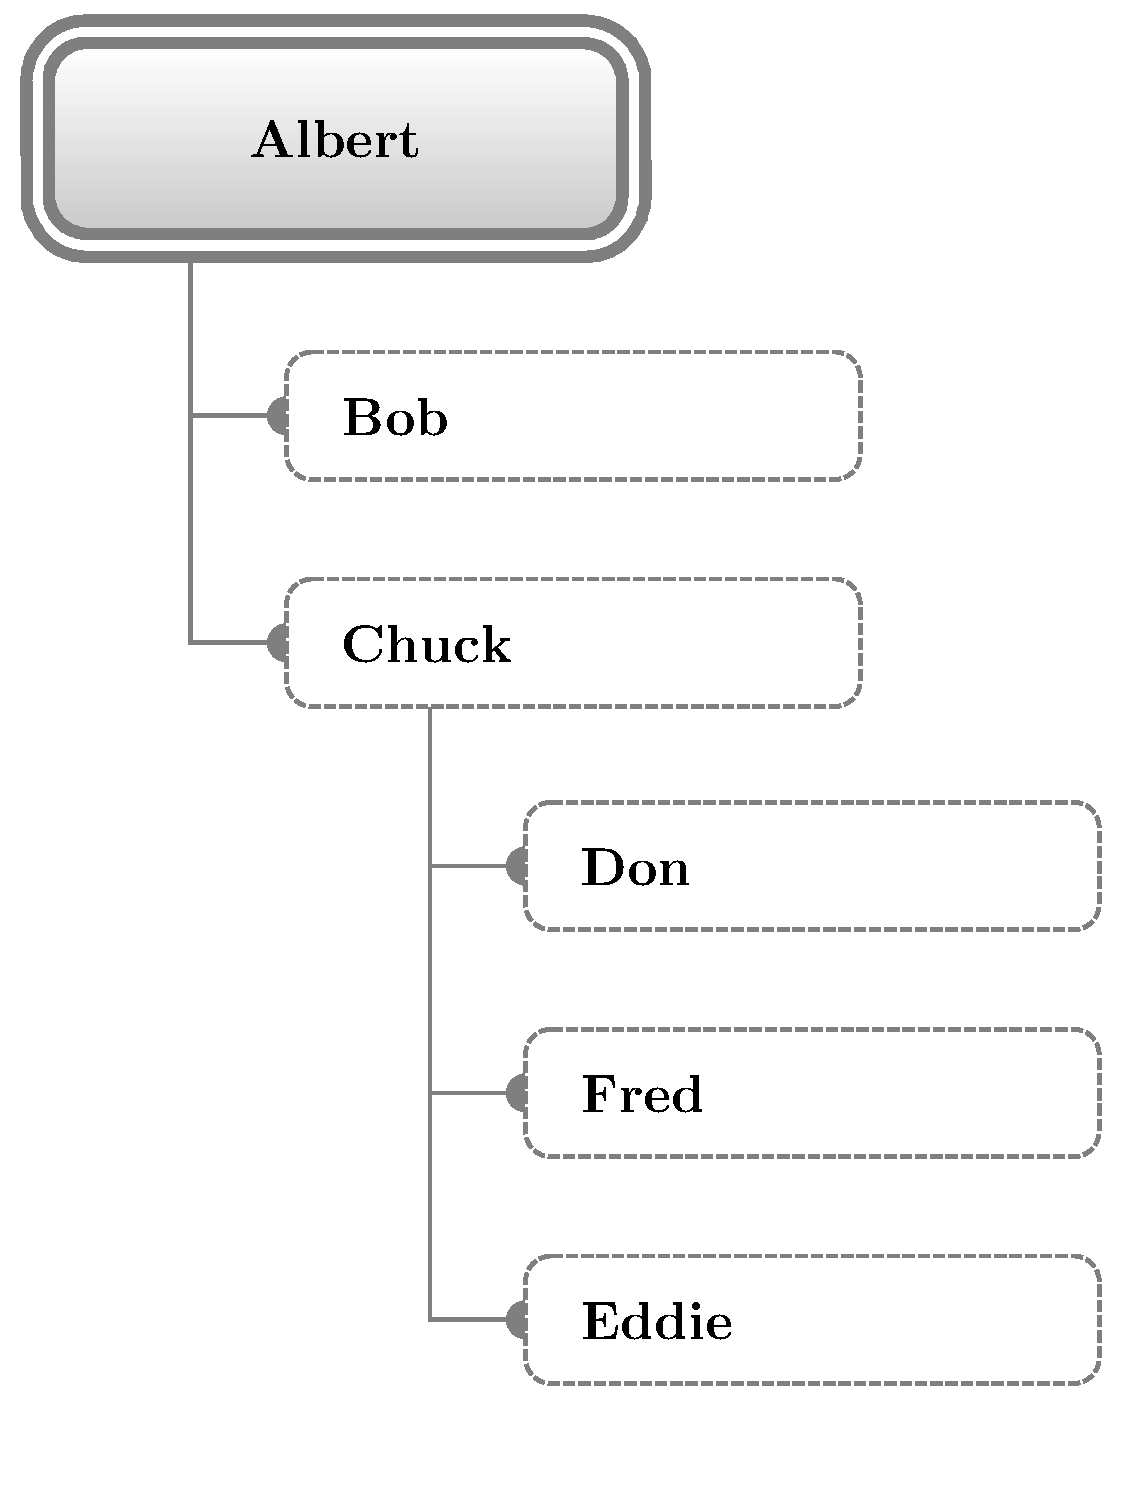
\includegraphics[width=5cm]{graphics/02-strom}
\caption{Ukázkový strom}\label{fig:stri}
\end{figure}

\begin{table}
\centering
\caption{Hranová reprezentace stromu}\label{tab:str1}
\begin{tabular}{c | c}
id & rodič \\
\hline
Albert & Albert (nebo NULL) \\
Bob & Albert \\
Chuck & Albert \\
Don & Chuck \\
Fred & Chuck \\
Eddie & Chuck
\end{tabular}
\end{table}

Vidíme, že pokud jsou hodnoty v obou sloupcích shodné nebo je hodnota ve sloupci \textit{rodič} rovna hodnotě NULL, pak je daný uzel kořenem stromu. Již letmým pohledem vidíme, že tabulka obsahuje relativně minimum dat a nedá se z ní vyčíst například, zda Chuck je levým nebo pravým potomkem Alberta. Implementace vyhledávacího stromu je tedy prakticky nemožná.

%% TODO: Obrázek stromu

\subsubsection{Cestová reprezentace}
V cestové reprezentaci je pro každý uzel popsána jeho úplná cesta napříč celým stromem. V tomto případě je nejlepší pohled na tabulku \ref{tab:str2}, která způsob reprezentace dokonale vystihuje.

\begin{table}
\centering
\caption{Cestová reprezentace stromu}\label{tab:str2}
\begin{tabular}{c | c}
id & cesta \\
\hline
Albert & /Albert \\
Bob & /Albert/Bob \\
Chuck & /Albert/Chuck \\
Don & /Albert/Chuck/Don \\
Fred & /Albert/Chuck/Fred \\
Eddie & /Albert/Chuck/Eddie
\end{tabular}
\end{table}

Na procházení takto reprezentovaného stromu se hodí operátor\upinlinecode{SQL}{!}{LIKE} z \upabbrevref{SQL}.

\subsubsection{Reprezentace vnořenými množinami}
Speciální reprezentace, která se již neřadí mezi naivní, nýbrž pokročilé. Využivá v podstatě kombinace preorder a postorder průchodů stromem, kdy se každý uzel ohodnocuje dvojicí čísel, které popisují jeho \enquote{pořadí} ve stromu. Více napoví tabulka \ref{tab:str3}.

\begin{table}
\centering
\caption{Reprezentace stromu vnořenými množinami}\label{tab:str3}
\begin{tabular}{c | c c}
id & lt & rt \\
\hline
Albert & 1 & 12 \\
Bob & 2 & 3 \\
Chuck & 4 & 11 \\
Don & 5 & 6 \\
Fred & 7 & 8 \\
Eddie & 9 & 10
\end{tabular}
\end{table}

Bystré oko čtenáře vidí, jak se strom tímto způsobem \enquote{ohodnocuje}. Hodnoty atributů \textit{lt} a \textit{rt} odhalují vlastnosti a umístění jednotlivých uzlů ve stromů.

\begin{upexample}[Dotazy na části množinově reprezentovaného stromu]
Vidíme, že kořen má zvláštní hodnotu ve sloupci \textit{lt}.

\begin{upcode}{Dotaz na kořen stromu v množinové reprezentaci}{}{SQL}
SELECT * FROM tree WHERE lt = 1;
\end{upcode}

Také listy mají poněkud unikátní vztah mezi oběma hodnotami.
\begin{upcode}{Dotaz na listy stromu v množinové reprezentaci}{}{SQL}
SELECT * FROM tree WHERE lt = rt - 1;
\end{upcode}

Velkou zbraní této reprezentace je určení podstromu určitého uzlu.
\begin{upcode}{Dotaz na podstrom stromu v množinové reprezentaci}{}{SQL}
SELECT	tree_1.id AS from_node, tree_2.id AS to_node
FROM	tree AS tree_1, tree AS tree_2
WHERE	tree_2.lt BETWEEN tree_1.lt AND tree_1.rt;
\end{upcode}
\end{upexample}
